\tunemarkup{coverimage}{%
\newcommand{\adjustimg}{\checkoddpage\ifoddpage\hspace*{\dimexpr\evensidemargin-\oddsidemargin}\else\hspace*{-\dimexpr\evensidemargin-\oddsidemargin}\fi}
\newcommand{\centerimg}[2][width=\textwidth]{\makebox[\textwidth]{\adjustimg\includegraphics[#1]{#2}}}
\newpagecolor{ubpagecolor}\afterpage{\restorepagecolor}
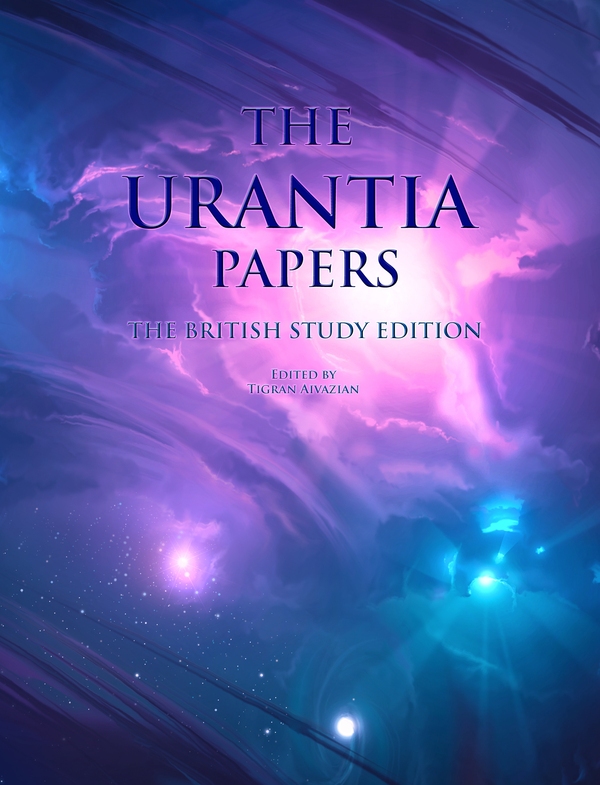
\includepdf{images/British-Study-Edition-Cover-tiny.png}
}

\makeatletter
\bib@raise@anchor{\bibpdfbookmark[0]{Title Page}{Ttl}}%
\makeatother

\vspace*{\stretch{0.1}}
\begin{center}
{
\bibcovertitlefont
\tunemarkup{pgcrownq}{\fontsize{25}{34}\selectfont}
\tunemarkup{pgafour}{\fontsize{27}{34}\selectfont}
\tunemarkup{pgkindledx}{\fontsize{20.8}{32}\selectfont}
\tunemarkup{pghanlin}{\fontsize{12}{20}\selectfont}
\tunemarkup{pgkobomini}{\fontsize{14}{20}\selectfont}
\tunemarkup{pgnexus7}{\fontsize{13.5}{20}\selectfont}
\tunemarkup{pgthinmob}{\fontsize{13.5}{20}\selectfont}
\tunemarkup{pgnexus10}{\fontsize{17.3}{28}\selectfont}
\tunemarkup{pgkoboaurahd}{\fontsize{15}{20}\selectfont}
\tunemarkup{pgauraone}{\fontsize{16.5}{20}\selectfont}
THE BRITISH \tunemarkuptwo{nofnt}{TEXT}{STUDY} EDITION\\
\tunemarkup{pgcrownq}{\fontsize{24}{34}\selectfont}
\tunemarkup{pgafour}{\fontsize{24}{34}\selectfont}
\tunemarkup{pgkindledx}{\fontsize{16.5}{32}\selectfont}
\tunemarkup{pghanlin}{\fontsize{9}{20}\selectfont}
\tunemarkup{pgkobomini}{\fontsize{10}{20}\selectfont}
\tunemarkup{pgnexus7}{\fontsize{10}{20}\selectfont}
\tunemarkup{pgthinmob}{\fontsize{10}{20}\selectfont}
\tunemarkup{pgnexus10}{\fontsize{14}{28}\selectfont}
\tunemarkup{pgkoboaurahd}{\fontsize{12}{20}\selectfont}
\tunemarkup{pgauraone}{\fontsize{12}{20}\selectfont}
OF\\
\tunemarkup{pgcrownq}{\fontsize{30}{38}\selectfont}
\tunemarkup{pgafour}{\fontsize{32.5}{38}\selectfont}
\tunemarkup{pgkindledx}{\fontsize{25}{32}\selectfont}
\tunemarkup{pghanlin}{\fontsize{9}{20}\selectfont}
\tunemarkup{pgkoboaurahd}{\fontsize{20}{23}\selectfont}
\tunemarkup{pgauraone}{\fontsize{20}{22}\selectfont}
\tunemarkup{pgkobomini}{\fontsize{16.6}{20}\selectfont}
\tunemarkup{pgnexus7}{\fontsize{16}{20}\selectfont}
\tunemarkup{pgthinmob}{\fontsize{16}{20}\selectfont}
\tunemarkup{pgnexus10}{\fontsize{23}{30}\selectfont}
\urantiapapers\\
}%
{%
\vspace*{\stretch{0.1}}
\tunemarkup{pghanlin}{\fontsize{10}{13}\selectfont}
\tunemarkup{pgkindledx}{\fontsize{16}{18}\selectfont}
\tunemarkup{pgcrownq}{\fontsize{19}{24}\selectfont}
\tunemarkup{pgafour}{\fontsize{21}{24}\selectfont}
\tunemarkup{pgnexus7}{\fontsize{10}{12}\selectfont}
\tunemarkup{pgthinmob}{\fontsize{10}{12}\selectfont}
\tunemarkup{pgnexus10}{\fontsize{15}{22}\selectfont}
\tunemarkup{pgkoboaurahd}{\fontsize{13}{17}\selectfont}
\tunemarkup{pgauraone}{\fontsize{13}{15}\selectfont}
\itshape
The Revised Text in British English\tunemarkuptwo{nofnt}{\\[2ex]}{%
,\\
with Metric Measures, \totalnfncs\ Textual Variants,\\
\totalnfnsts\ Study Notes \&\ \totalfigures\ Illustrations\\[2ex]
}
\tunemarkup{pgnexus7}{\textcolor{ubdarkred}{With Words of Jesus in Red Colour}\\[1pt]}
Edited by Tigran Aivazian\\[2ex]
\tunemarkuptwo{noquiz}{}{With Interactive Cosmic Citizenship Quiz\\(\totalcurqs\ questions in total)\\}
}%
\ifmultivol
\LARGE\bfseries\itshape
\ifvoli Volume I: Foreword \&\ Papers 1--96\\\fi
\ifvolii Volume II: Papers 97--196\\\fi
%\ifvoliii Volume III: Papers 129--196\\\fi
\fi
\vspace*{\stretch{0.6}}
\titlesepbig\\
\vspace*{\stretch{0.1}}
\end{center}

\titleframe

\newpage

%\newcommand{\serpimolot}{{\fontspec{Mortbats} K}}

\begin{center}
\vspace*{\stretch{0.3}}
\begin{center}\shadowbox{\strut\parbox{7cm}{\normalsize\tunemarkup{pgnexus10}{\large}\tunemarkup{pgkindledx}{\Large}\tunemarkup{pgcrownq}{\Large}\tunemarkup{pgafour}{\large}\bfseries\itshape ``Of all human knowledge, that which is of greatest value is to know the religious life of \mbox{Jesus} and how he lived it.'' \bibref[(196:1.3)]{p196 1:3}}}\end{center}
\vspace*{\stretch{0.5}}
\tunemarkup{pghanlin}{\fontsize{8}{10}\itshape}
\tunemarkup{pgkobomini}{\fontsize{9}{10}\itshape}
\tunemarkup{pgnexus7}{\fontsize{8}{10}\itshape}
\tunemarkup{pgthinmob}{\fontsize{8}{10}\itshape}
\tunemarkup{pgnexus10}{\fontsize{12}{16}\itshape}
\tunemarkup{pgkindledx}{\fontsize{10}{12}\itshape}
\tunemarkup{pgcrownq}{\Large\itshape}
\tunemarkup{pgafour}{\Large\itshape}
\parbox{0.9\linewidth}{\centering
\textbf{\upshape\nocopyright\ No copyright is claimed on this book\\
The text of \bibemph{The Urantia Papers} is in the public domain.}\\[5pt]
\tunemarkuptwo{coverimage}{Cover design by Gary Tonge.\\}{}
The latest version of this book can be downloaded from:\\
{\upshape\bfseries http://www.bibles.org.uk}\\
Please send all comments to: {\makeatletter\upshape\bfseries aivazian.tigran@gmail.com\makeatother}\\[1ex]
\tunemarkuptwo{pgafour}{}{\small}\tux\ Typeset with \XeLaTeX\ of \TeX\ Live 2017 under Linux.\\
Text set in \textbf{\itshape\tunemarkup{minionpro}{Adobe }\tunemarkup{garamond}{Adobe }\tunemarkup{arno}{Adobe }\tunemarkup{academy}{ParaType }\urantiamainfont} at \urantiamainfontsize pt.\\[18pt]
\upshape\small\tunemarkup{pgcrownq}{\large}\tunemarkup{pgafour}{\Large}\bfseries PDF version: \tunemarkup{pgthinmob}{20:9 Colour}\tunemarkup{pgcrownq}{Crown Quarto}\tunemarkup{pgafour}{A4}\tunemarkup{pgnexus7}{7" Colour}\tunemarkup{pgnexus10}{10" Colour}\tunemarkup{pghanlin}{6" eInk}\tunemarkup{pgkobomini}{5" eInk}\tunemarkup{pgkoboaurahd}{7" eInk}\tunemarkup{pgkindledx}{10" eInk}\tunemarkup{pgauraone}{8" eInk}\\
\upshape\bfseries PDF date: \mytoday{}\\
}
\vspace*{\stretch{0.1}}
\end{center}

\titleframe
